% Use xelatex
% chktex-file 24
\documentclass{hse_document}

\begin{document}

\maketoc{КОМПОНЕНТЫ ПРОГРАММНОЙ СИСТЕМЫ}{Отчёт по лабораторной работе}{В.П. Куприн}

\tableofcontents
\clearpage

\addcontentsline{toc}{section}{Введение}
\section*{Введение} \label{Введение}

\textbf{Название работы:}
Лабораторная работа №3 <<Компоненты программной системы.>>

\textbf{Цель работы:}
Научиться выделять подсистемы программной системы,
определять связи между ними.

\textbf{Ожидаемый результат:}
Диаграмма компонентов (СОМРОNЕNТ) с текстовым описанием.

\section{Компоненты программной системы}\label{sec:components}

Среди компонентов программной системы необходимо выделить следующие:

\begin{compactenum}
\item Клиента, который создаёт запросы к API;
\item Компонент обработки этих запросов. Он будет обращаться к БД за данными и к
    модулю Машины состояний для проведения всех вычислений;
\item Компонент базы данных;
\item Компонент машины состояний. Исходя из переданных данных он вычисляет
    состояние машины.
\end{compactenum}

Диаграмма компонентов представлена на Рисунке \ref{fig:components}.

\begin{figure}[htpb]
    \centering
    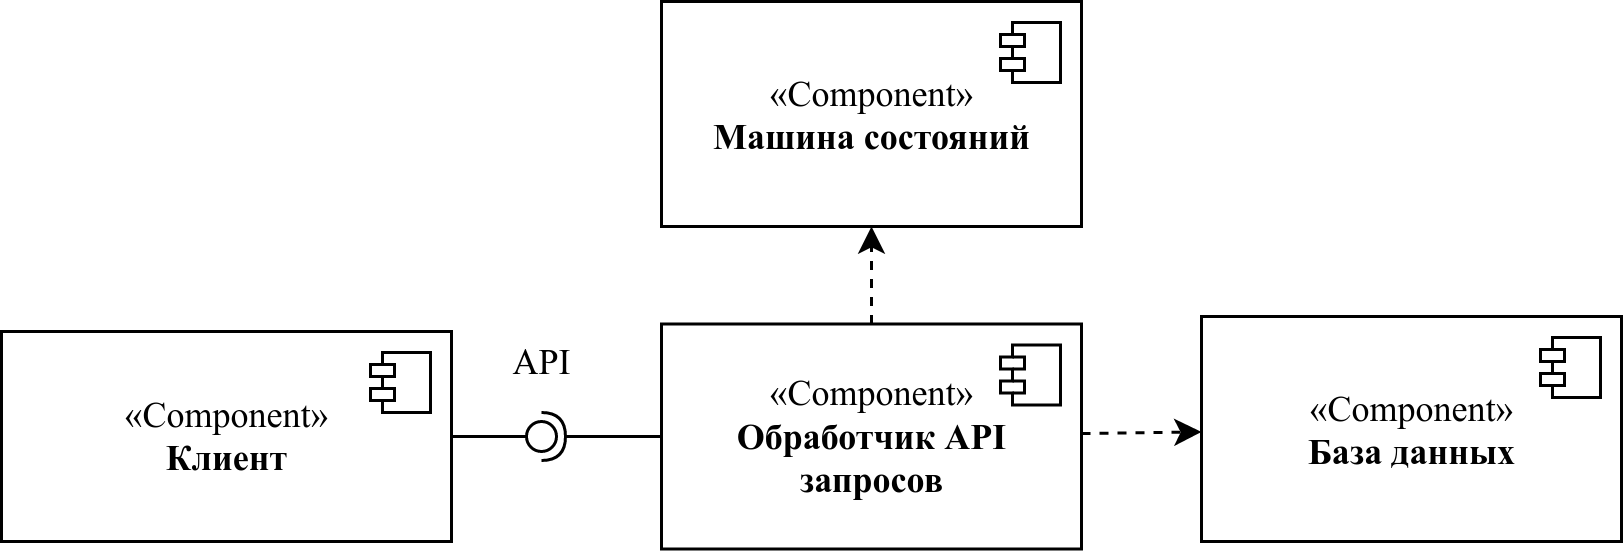
\includegraphics[width=0.8\textwidth]{diagrams/components.png}
    \caption{Диаграмма компонентов}
    \label{fig:components}
\end{figure}


\section{Данные}

Машина состояний должна иметь набор возможных состояний.
Состояния будут задаваться числовыми идентификаторами.
Правила возможных переходов будут определяться парами <<начальное состояние>>
--- <<конечное состояние>>.

Условия для осуществления переходов будут задаваться в виде предикатов.
Пример предиката с точки зрения пользователя: <<Значение показателя X стало
больше отметки Y>>. Будут реализованы следующие типы предикатов:

\begin{compactitem}
\item Больше;
\item Больше или равно;
\item Равно;
\item Не равно;
\item Меньше;
\item Меньше или равно.
\end{compactitem}

Таким образом, базовые предикаты должны хранить информацию о свойстве объекта,
типе предиката, значении для сравнения (фиксированное или же значение
какого-либо свойства объекта).

Выделим сущности системы:
\begin{compactitem}
\item Пользователь;
\item Машина состояний: содержит список состояний, идентификатор, список
    возможных переходов и их правила, описание объекта;
\item Объект (типы полей и их значения);
\item Правила переходов (свойство, оператор сравнения и значение для сравнения);
\item Изменение --- набор изменённых полей объекта;
\item Событие (идентификатор).
\end{compactitem}

Построим ER-диаграмму. Результат представлен на Рисунке \ref{fig:erd}.

\begin{figure}[htpb]
    \centering
    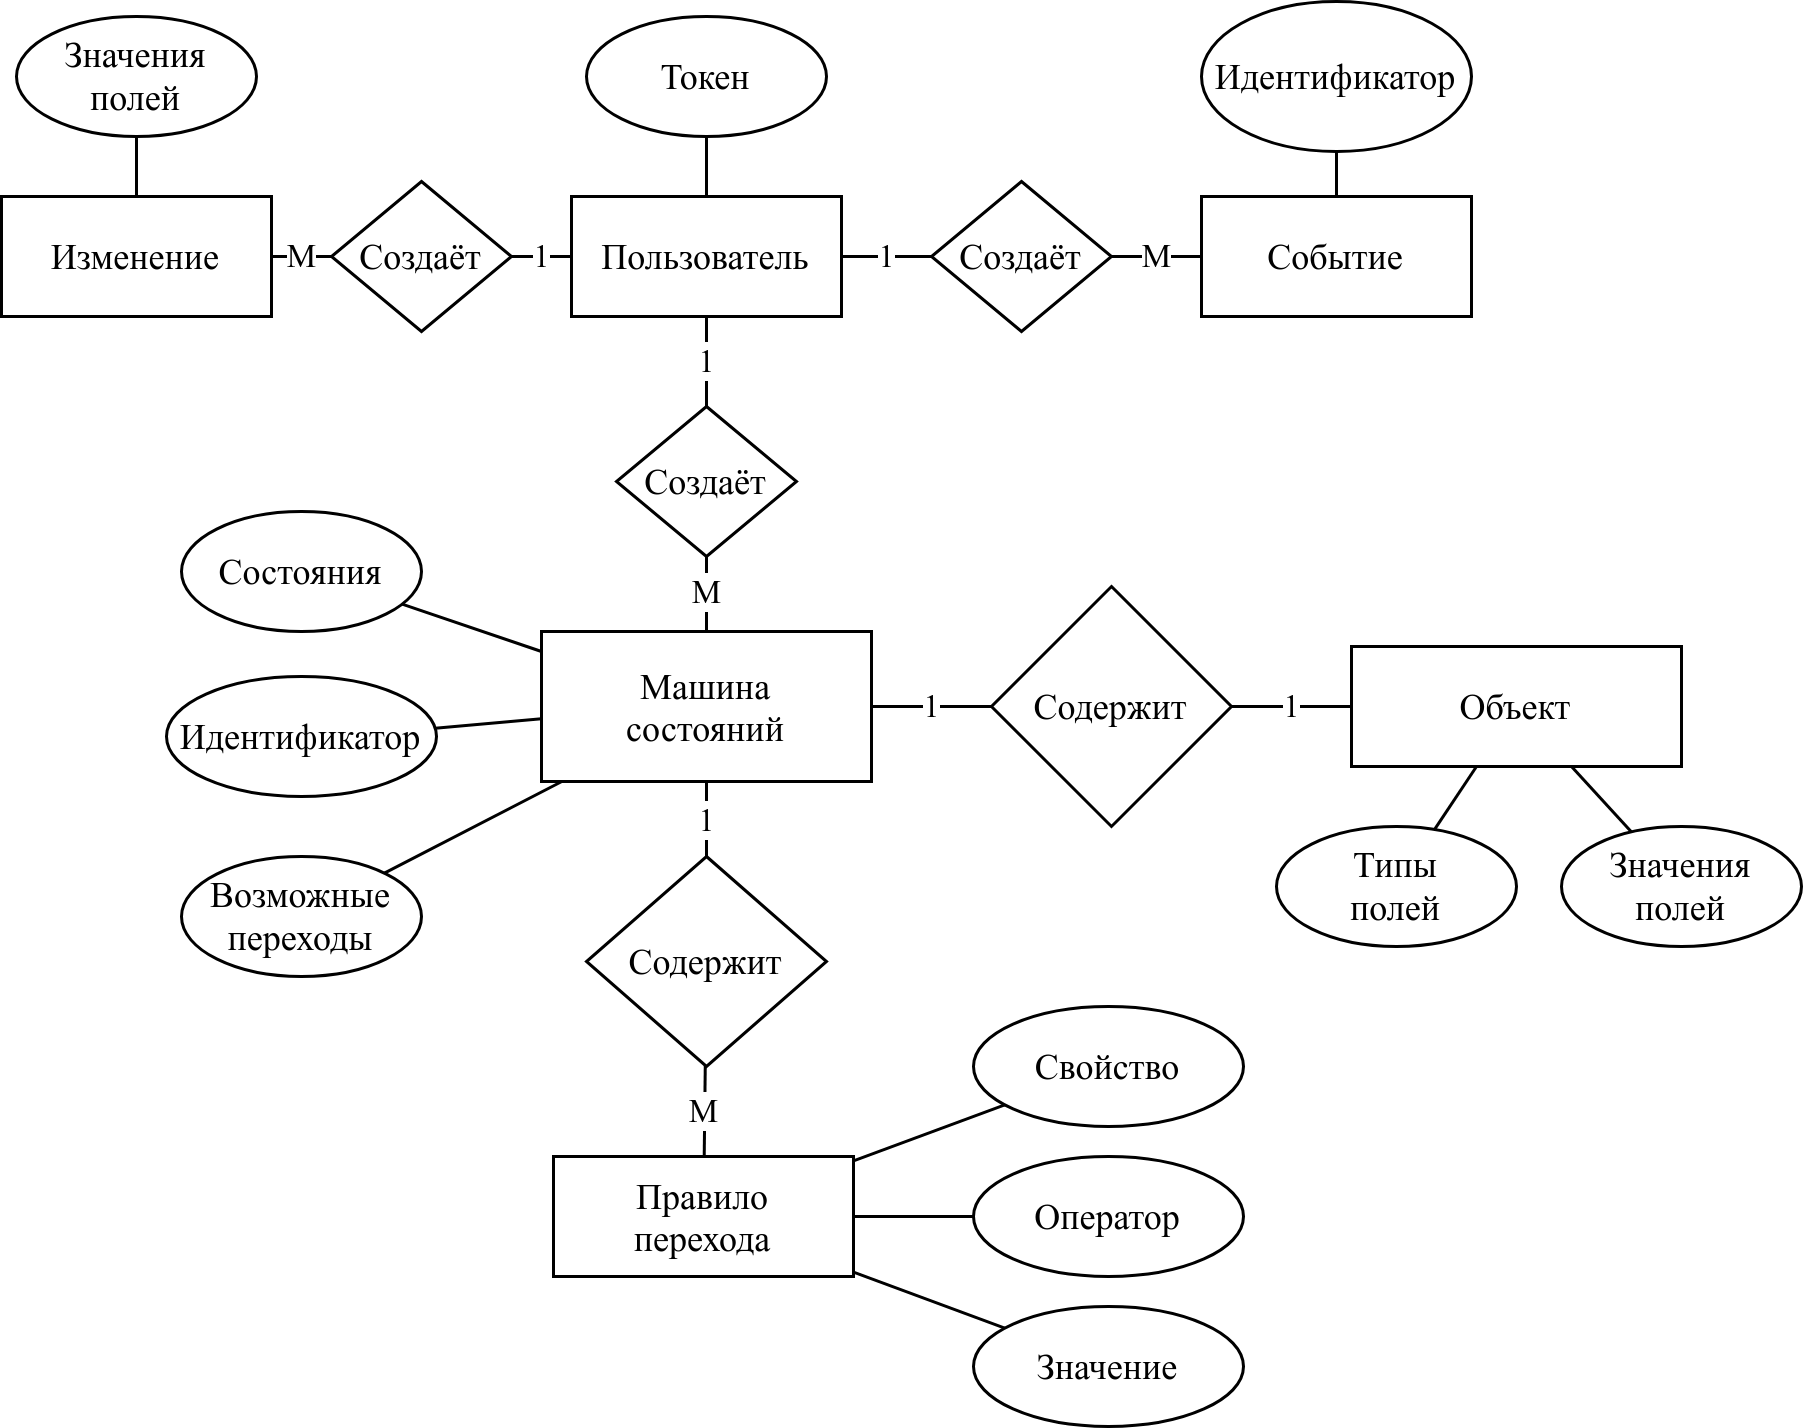
\includegraphics[width=0.9\textwidth]{diagrams/erd.png}
    \caption{Entity Relationships Diagram}
    \label{fig:erd}
\end{figure}



\end{document}
